\graphicspath{{figures/figures_eqcosmo/}}


\section{Chapter Abstract}
The laws of physics obey exact symmetry properties.
The method of invariant scalars is a lightweight and physically motivated way to encode these symmetries in analysis methods, by compressing inputs into scalars that are invariant to rotations, translations, and permutations (particle labeling).
We apply this approach to analyze the relationship between dark matter (DM) and baryons in cosmological simulations, which is critical for understanding the galaxy--halo connection and inferring cosmological parameters from large-scale structure.
Using IllustrisTNG simulation data, we build a training set consisting of DM halos in the DM-only simulation and their corresponding central galaxies in the matched hydrodynamical simulation. 
For each DM halo, we construct a large set of invariant scalars based on geometric phase-space properties of the DM particle distribution.
With these scalars as inputs, we use a neural network to predict the properties of the corresponding galaxies, most importantly the stellar mass.
We show that our approach outperforms the use of standard halo summary properties as the features, as well as using the same geometric information but not compressed into invariant quantities.
The exact symmetries inherent to our method impose informative constraints while preserving the known invariance properties of large-scale structure.
Further, our results are interpretable in terms of the information in DM phase-space and give insight into the connection between galaxy and DM halo properties, relevant to open questions in galaxy formation including the importance of assembly bias on the galaxy--halo connection.


\section{Introduction}

One of the key goals of modern galaxy redshift surveys is to infer the cosmological parameters that govern the composition and evolution of the universe.
In order to perform this inference, we need to model the galaxy distribution; we do so using massive simulations of the cosmic web.
These N-body simulations, however, only evolve dark matter (DM) particles gravitationally. 
Hydrodynamic simulations to simulate galaxies are much more expensive, so often DM-only simulations are run and then ``populated'' with galaxies post-facto, using empirically motivated models.

The goal of this work is to use a theoretically motivated approach to populate DM-only simulations with galaxies.
We propose an approach that enforces the known symmetries of cosmological simulations, including translational and rotational symmetry, when mapping DM halos to galaxy properties.
We use the method of \emph{invariant scalars} \citep{Villar2021a}, which represents equivariant functions using a collection of scalar quantities, directly incorporating symmetry preservation into prediction tasks.

In this work, we use the following notation: 
Scalars are denoted by lowercase variables, vectors by lowercase bold variables, and tensors by uppercase bold variables.
\ksf{etc}

This paper is outlined as follows.
In \S\ref{sec:sim_sample}, we introduce the simulation used and our sample selection. 
In \S\ref{sec:methods}, we describe the invariant scalars approach and our linear regression model.
In \S\ref{sec:results}, we present the results of predicting galaxy properties from DM halo features, and in \S\ref{sec:discussion}, we interpret these results and discuss their implications and applications.


\section{Simulation and Sample Construction}
\label{sec:sim_sample}

\subsection{The IllustrisTNG simulations}
\label{sec:tng}

The Illustris TNG simulations are cosmological magnetohydrodynamical simulations that co-evolve dark matter and baryons to model galaxy formation \citep{springel_first_2018,nelson_first_2018,pillepich_simulating_2018,naiman_first_2018,marinacci_first_2018}.\footnote{Data products from the TNG Project are publicly accessible at \url{https://www.tng-project.org/}.}
The simulations are run starting from initial conditions at $z=127$ with cosmological parameters from \cite{ade_planck_2016} $\Omega_m = \Omega_{dm} + \Omega_b = 0.3089$, $\Omega_b = 0.0486$, $\Omega_\Lambda = 0.6911$, Hubble constant $H_0 = 100$ $h$ km s$\inv$ Mpc$\inv$ with $h = 0.6774$, $\sigma_8 = 0.8159$, and $n_s = 0.9667$.
They model baryonic processes including ionizing background radiation, star formation and stellar feedback, stellar evolution and chemical enrichment, pressurization of the interstellar medium from supernovae, and the growth of and feedback from supermassive black holes.   
We use the TNG-100-1 simulation, which has a size of $L = (75 \hMpc)^3$, $1820^3$ DM particles and the same number of gas cells, and mass resolutions of $m_\text{DM} = 7.5 \times 10^6 \Msun$ and $m_\text{gas} = 1.4 \times 10^6 \Msun$.
The simuluation also evolves star/wind and black hole particles.
It has a matched DM-only simulation run with the same initial conditions, TNG-100-1-Dark, with mass resolution of $8.9 \times 10^6 \Msun$.
We refer to the DM-only simulation (TNG-100-1-Dark) as \dark and the hydrodynamical simulation (TNG-100-1) as \hydro in the rest of this work.
For most of this work, unless otherwise stated, we use the $z=0$ snapshot.

We use the DM halo catalogs provided by the TNG project as the starting point for our sample.
Halos are defined by a Friends-of-Friends (FoF) algorithm on DM particles, with a linking length of 0.2 times the mean inter-particle separation; other types of particles are assigned to the same halo as their nearest DM particle.
Subhalos within halos are found using the Subfind algorithm, which identifies gravitationally bound structures across all particle types.


\subsection{Halo and galaxy sample selection}
\label{sec:select}

One of our goals with this project is to propose a characterization of DM halos that is useful for predicting the properties of the galaxies they host, as well as their assembly history.
Given this, we operate on the halos in the \dark (DM-only) simulations, with the idea of learning the results of the hydrodynamic galaxy formation model.
To that end, we construct a sample of paired DM halos in the \dark simulation and galaxies in the \hydro (full hydrodynamical) simulation. 
We consider only central galaxies in this work; the approach could be straightforwardly extended to satellite galaxies.

We first make a cut on the \dark halos, choosing only halos with a mass $\Mfof > 10^{10.25} \, \hMsun$, where $\Mfof$ is the mass of all the particles that are part of the FoF group within $\Rtwoh$, and $\Rtwoh$ is the radius enclosing a mass of 200 times the mean density of the simulation.
We use this mass definition, as opposed to the typical $\Mtwoh$ which includes all particles both part of and not part of the FoF group, as our approach will operate only on the FoF particles and this keeps the mass definitons consistent; however, this is just for technical reasons, and only differs at the few percent level.
We require that the halos have at least one subhalo.
We use the matched subhalo catalogs provided by the TNG Project, which match subhalos in the dark simulation to subhalos in the paired hydrodynamical simulation; we call these subhalo pairs ``twins''.
The matching is done with the ``LHaloTree'' algorithm, which selects the halo in the other simulation with the largest number of DM particles in common, and requires that both simulations agree, resulting in bijective matches.
We discard halos that do not have a \hydro match.
For every \dark halo, we take its most massive \dark subhalo.
For that \dark subhalo, we find its twin \hydro subhalo.
We consider the baryons in this subhalo to constitute the central galaxy that is associated with the original \dark halo; we call this the ``matched'' galaxy of the \dark halo. 
We note that this twin \hydro subhalo is nearly always (but occasionally not) the most massive subhalo in its parent halo in the \hydro simulation.

We make some additional cuts on this sample.
We note that some of these cuts are on the ``labels'' or otherwise require knowledge of the hydrodynamical simulation; in a full application this should be handled more carefully, such as implementing an additional prediction step. 
We discard all \dark halos for which the twin \hydro subhalo has fewer than 50 star particles.
We discard all pairs for which the mass $\Mtwoh$ of the DM halo and the matched hydro halo differ by a factor of 3 or more; we assume that this indicates a bad match, and only occurs for a very small fraction of halos.
We also require that the SC-SAM has been applied to the halos, as we use the halo assembly histories computed by the SC-SAM (discussed further in \S\ref{sec:mah}); this removes a few percent of the halos.
These selections result in XXX \dark halos and matched \hydro galaxies.
We use 70\% as a training set, 15\% as a validation set, and 15\% as a test set.


\subsection{Halo mass assembly history}
\label{sec:mah}

We aim to predict the mass assembly history of the \dark halos based only on their present-day ($z=0$) properties.
This is informative as it captures the dynamical history of the halo, which affects the formation of the galaxies it hosts.
We use the merger histories computed by \citep{gabrielpillai_galaxy_2021} as part of a comparative analysis between TNG and the Santa Cruz semi-analytic model (SC-SAM, \citealt{somerville_semi-analytic_1999,somerville_semi-analytic_2008, somerville_star_2015}); the SAM is based on these merger trees.\footnote{The merger history and other SC-SAM data is publicly accessible at \url{https://github.com/aust427/illustris_sam}.}
The merger trees are run on halos found with the \textsc{rockstar} \citep{behroozi_rockstar_2013} code and built with \textsc{consistent trees} \citep{behroozi_gravitationally_2012}, and a bijective matching is performed between the \textsc{rockstar} and TNG Subfind halos.

We consider the most massive progenitor branch of the assembly history of each \dark halo in our sample.
We compile the mass of the halo's most massive progenitor for each of the TNG snapshots. 
A natural quantity to try to predict would be the fraction of the $z=0$ halo mass accreted as a function of redshift.
However, different halos can be traced back to different redshifts, and this inconsistency causes difficulties at the prediction stage.
We thus choose to learn the scale factor $a$ (related to the redshift $z$ by $a=1/(1+z)$) at which the halo has accreted a given fraction of its mass, $M_\mathrm{vir}(a)$/$M_\mathrm{vir}(a=1)$, where $M_\mathrm{vir}$ is given by the \texttt{HalopropMvir} field of the SC-SAM data and $a=1$ is the present day.
This swapped quantity gets at the same information as the natural quantity but is more stable in predictions.
We compute this at XXX linearly spaced mass fractions between 0 and 1 (exclusive). 
As we only have the history at a finite number of snapshots, we perform a linear interpolation between the mass fractions and scale factors to estimate the scale factor at a given mass fraction.
If the target mass fraction is outside the bounds of the data (for example, if the initial mass of the halo was a larger mass fraction than our tabulated values), we assign the scale factor to be that at which the mass fraction is closest.  



\subsection{Galaxy properties and uncertainties}
\label{sec:galprops}




\section{The invariant scalars approach}
\label{sec:methods}

Our approach for mapping the halo particle distribution to galaxies uses the ``scalars'' approach of \cite{Villar2021a}.
The core idea is that functions equivariant to certain transformations can be expressed in terms of a set of scalars, constructed from the input quantities.  
Motivated by the fact that the physical laws that govern cosmological simulations obey exact symmetries, specifically translation, rotation, and permutation (of the particles), we apply the scalars approach to the particle distribution of dark matter halos with the goal of performing prediction tasks.
Specifically, we use a multipole expansion to compress the particle positions and velocities of each halo into a set of ``geometric features'' that describe the phase-space structure of the halo; this is discussed in \S\ref{sec:geometric_features}.
We then construct scalar contractions of these geometric features, which are scalars, vectors, and tensors, and these ``scalar features'' are invariant to transformations of the particles. 
This step is informed by Einstein summation notation, which only allows invariant scalars to be produced; the details of our scalar feature construction is discussed in \S\ref{sec:scalar_features}.
We can finally use these scalar features as the inputs for our prediction task; in our case we perform a linear regression on them (\S\ref{sec:regression}), though they could also be used with other models such as neural networks.

In contrast, typical approaches use a small set of hand-constructed properties of the halos; while these do often obey physical symmetries, this is not enforced, and the properties do not necessarily capture the complexity of the halos, in particular their phase-space structure.
A maximalist approach could use the full particle distribution, but this is prohibitively expensive and would not obey the known symmetries.
The scalars approach allows for a flexible, lightweight set of halo features that respects symmetries and provides a more complete representation of halos.
We also expect the enforced equivariance to make the approach more generalizable, for instance to different resolutions or simulation codes.

\subsection{The physical symmetries}
\label{sec:symmetries}

% to write
%what is a geometric object? scalars, vectors, tensors - defined by their transformation properties under rotation, translation, permutation. properties that ensure that coordinate freedom preserve angular momentum, linear momentum, etc

\subsection{Geometric features}
\label{sec:geometric_features}

\begin{table}
    \caption{The geometric features we construct from the dark halo particles, following the multipole expansion of \refeq{eq:geo}. The table gives, for each feature, its name, its orders in mass, position, and velocity, and its interpretation.  \ksf{better name for covariance object?} \ksf{how to sort? be consistent w how i do for feature importance! m, x+v, v, x? (now not doing x+v, and doing x, v - confusing what makes sense)}}
    \label{tbl:geometric_features}
    \vspace{0.5em}
    \centering
    \begin{tabular}{|l|l|l|l|l|l|}
    \hline
    moment & name & $O(m)$ & $O(\x)$ & $O(\vel)$ & interpretation \\
    \hline
    $g_{00n}$ & $m_n$ & 1 & 0 & 0 & mass in $n$th bin \\
    $g_{10n}$ & $\langle \x \rangle_n$ & 1 & 1 & 0 & mass-weighted position of $n$th bin \\
    $g_{01n}$ & $\langle \vel \rangle_n$ & 1 & 0 & 1 & mass-weighted velocity of $n$th bin \\
    $g_{20n}$ & $C^{(\x\x)}_n$ & 1 & 2 & 0 & variance tensor of positions in $n$th bin \\
    $g_{11n}$ & $C^{(\x\vel)}_n$ & 1 & 1 & 1 & covariance of positions and velocities in the $n$th bin \\
    $g_{02n}$ & $C^{(\vel\vel)}_n$ & 1 & 0 & 2 & variance tensor of velocities in $n$th bin \\
    \hline
    \end{tabular}
\end{table}

We first compute a set of ``geometric features'' from our data from the particle distribution, using their masses, positions, and velocities. 
We choose the geometric features to be based on a multipole expansion, computing moments of the data in a set of radial shells. 
The geometric features $g_{\ell p n}$ are: 
\label{eq:geo}
\begin{equation}
    g_{\ell p n} = \sum_i m_i W_n(r_i)  \left[ \x_i^{\otimes \ell} \, \otimes \, \vel_i^{\otimes p} \right]
\end{equation}
where $i$ indexes the particle, $m_i$ is the mass of the $i$th particle, $W_n(r_i)$ is the $n$th window function, and $r_i$ is the distance between the position of the $i$th particle and some fiducial point.
We choose this fiducial point, which functions as the halo center, to be the location of the most bound particle in the halo (the particle with the minimum potential energy).
The quantity $x_i^{\otimes \ell}$ is the $\ell$th moment (outer product $\ell$ times) of the particle position (with respect to the fiducial point); for $\ell = 1$, this is just the position of the particle.
The quantity $v_i^{\otimes p}$ is the same but for the velocities, where the velocities are with respect to the center of velocity of all the particles in the halo.
We see that $g_{00n}$ are scalars, $g_{01n}$ and $g_{10n}$ are vectors, $g_{20n}$, $g_{02n}$, and $g_{11n}$ are tensors, and so on.
These geometric features have, at least at low order, interpretable meaning in terms of the halo shape.
For instance in the $n$th window, $g_{00n}$ is the mass of all the particles in that bin, $g_{10n}$ is their center of mass position, and $g_{20n}$ is their variance tensor.
\ksf{TODO: use fancy big O}

We make the following choices when computing our set of geometric features.
We compute the geometric features up to second order in position and velocity combined, $O(\x) + O(\vel) \leq 2$; this means we don't have objects of higher rank than a rank-2 tensor. 
We include cross-terms between position and velocity.
We use a top-hat window function producing hard-edged bins. 
Our bins are functions of each halos radius, given by $\Rtwoh$, the radius that encloses a mass of 200 times the mean density of the universe at that time.
Specifically we choose three bins that represent the inner part of the halo, the outer region but within $\Rtwoh$, and the outskirts of the halo: $n=0: [0, 0.375\Rtwoh]$, $n=1: [0.375\Rtwoh, \Rtwoh]$, $n=2: [\Rtwoh, \infty]$.
\ksf{figure out better notation here}
\ksf{for names, should even give in bins names, like inner, mid, outskirts?}
A full description of these geometric features and their orders can be found in Table~\ref{tbl:geometric_features}.

\subsection{Invariant scalar features}
\label{sec:scalar_features}

\begin{figure}
    \centering
    %\includegraphics{}
    \caption{A selection of dark matter halos of fixed mass (M=YYY), colored by the value of one of the invariant shape scalars, XXX. The central galaxy each one hosts is shown in the bottom row, colored by its stellar mass; the invariant scalar is correlated with the stellar mass, demonstrating how it is a useful predictor for the galaxy--halo connection.}
    \label{fig:halo_viz}
\end{figure}


\begin{table}
    \caption{All scalar polynomial features constructed from the geometric features, up to second order in $m$,  $O(m) \leq 2$, and fourth order in each of $\x$ and $\vel$, $O(\x) \leq 4$ and $O(\vel) \leq 4$. The indices $n$ and $n'$ index the radial bins of the geometric features, $q$ and $q'$ index the eigenvalues, and $j$ and $k$ are the indices summed over in Einstein summation notation. \ksf{Try to compute this table algorithmically in code? going to be tricky... but good check!} \ksf{eigenvalues in einstein notation??}} 
    \label{tbl:scalar_polynomials}
    \vspace{0.5em}
    \centering
    \begin{tabular}{|l|l|l|l|l|l|}
    \hline
    vector not. & summation not. & $O(m)$ & $O(x)$ & $O(v)$ \\
    \hline
    $g_{00n}$ & $g_{00n}$ & 1 & 0 & 0 \\
    %$\mathrm{Tr}(g_{20n})$ & $[g_{20n}]_{jj}$ & 1 & 2 & 0 \\
    $\lambda_q(g_{11n})$ & ? & 1 & 1 & 1 \\
    $\lambda_q(g_{20n})$ & ? & 1 & 2 & 0 \\
    $\lambda_q(g_{02n})$ & ? & 1 & 2 & 2 \\
    $g_{00n} \, g_{00n'}$ & $g_{00n} \, g_{00n'}$ & 2 & 0 & 0 \\
    $g_{00n} \, \lambda_q(g_{20n})$ & ? & 2 & 2 & 0 \\
    %$g_{00n} \, \mathrm{Tr}(g_{20n'})$ & $g_{00n} \, [g_{20n'}]_{jj}$ & 2 & 2 & 0 \\
    $g_{10n}\T \cdot g_{10n'}$ & $[g_{10n}]_j \, [g_{10n'}]_j$ & 2 & 2 & 0 \\
    $g_{10n}\T \cdot g_{01n'}$ & $[g_{10n}]_j \, [g_{01n'}]_j$ & 2 & 1 & 1 \\
    $g_{01n}\T \cdot g_{01n'}$ & $[g_{01n}]_j \, [g_{01n'}]_j$ & 2 & 0 & 2 \\
    $\lambda_q(g_{20n}) \, \lambda_{q'}(g_{20n'})$ & ? & 2 & 4 & 0 \\
    $ ? $ & $[g_{20n}]_{jk} \, [g_{20n'}]_{jk}$ & 2 & 4 & 0 \\
    $ ? $ & $[g_{20n}]_{jk} \, [g_{11n'}]_{jk}$ & 2 & 3 & 1 \\
    $ ? $ & $[g_{11n}]_{jk} \, [g_{11n'}]_{jk}$ & 2 & 2 & 2 \\
    $ ? $ & $[g^A_{11n}]_{jk} \, [g^A_{11n'}]_{jk}$ & 2 & 2 & 2 \\
    $ ? $ & $[g_{20n}]_{jk} \, [g_{02n'}]_{jk}$ & 2 & 2 & 2 \\
    $ ? $ & $[g_{11n}]_{jk} \, [g_{02n'}]_{jk}$ & 2 & 1 & 3 \\
    $ ? $ & $[g_{02n}]_{jk} \, [g_{02n'}]_{jk}$ & 2 & 0 & 4 \\
    \hline
    \end{tabular}
\end{table}

We can contract these geometric features to obtain ``polynomial features'' that will be the inputs to our model.
As our goal is to predict the mass of the galaxy, a scalar, we must only use scalar values as the input.
Our ``scalar features'' are then all allowed contractions of the geometric features that produce scalars. 
Broadly, scalars can be multiplied by other scalars; for vectors, one can take the outer product of it with another vector; and for tensors, one can perform a full contraction of it with another tensor, or take its trace or eigenvalues.
One natural way to neatly enumerate these scalars is using Einstein summation notation, as it only allows invariant scalars to be produced.
To construct a scalar, there must be no hanging indices, so we know that all indices used in the summation must be repeated.

We make some specific choices regarding the computed scalars.
We limit ourselves to certain orders in $m$, $\x$, and $\vel$, as the number of possible scalars expands greatly at higher order.
We choose to use the eigenvalues $\lambda_q$ of each tensor, where $q=1$ is the maximum eigenvalue, which gives more information than just the trace.
We include cross-terms across different bins $n$ and $n'$, and cross-terms between position and velocity geometric features (there is already a geometric term that depends on both position and velocity, $C^{\x \vel}$).
The allowed scalar contractions are shown in Table~\ref{tbl:scalar_features}.

One feature that we must handle specially is $g_{11n}$, which is the cross term of $\x$ and $\vel$, as the ordering of these terms matters
In this case, we can construct the symmetric feature $g^S_{11n} = \frac{1}{2} \sum_i m_i W_n(r_i) \left[ \x_i \, \otimes \, \vel_i + \vel_i \, \otimes \, \x_i \right]$ and the antisymmetric feature $g^A_{11n} = \frac{1}{2} \sum_i m_i W_n(r_i) \left[ \x_i \, \otimes \, \vel_i - \vel_i \, \otimes \, \x_i \right]$.
\ksf{better notation here?}
The antisymmetric feature is a pseudo-tensor, and the only way we can obtain a scalar is to contract it with another pseudo-tensor; which in our case will be another antisymmetric feature $g^A_{11n'}$.
The symmetric feature is a vector and can be treated like any other vector, so for conciseness we refer to $g^S_{11n}$ as simply $g_{11n}$.

We rescale our scalar features by overall halo quantities, so that the features are dimensionless and obey ``units symmetry''.
For every mass order, we scale the feature by the total mass of the halo, $\Mtot$; for every $\x$ order, we scale by the root-mean-square of the particle positions, $\xrms$; and for every $\vel$ order, we scale by the root-mean-square of the particle velocities.
We include these quantities as additional features, as described in \S\ref{sec:regression}.


\section{Prediction model}
\label{sec:regression}

To predict the desired output scalars, we train a fully collected neural network.


The neural net takes as input a set of scalar features as described in \S\ref{sec:scalar_features} for a given halo, along with the overall quantities used for rescaling, $\Mtot$, $\xrms$, and $\vrms$ (we take their logarithms to reduce the dynamic range).
The labels are the scalar galaxy properties of interest.
The NN consists of XXX layers, with SELU activation functions in between; we choose these because ... 

We use a Gaussian loss function, which takes the form
\begin{equation}
    L = 
\end{equation}
The uncertainties $\sigma$ on the labels are based on the intrinsic scatter as a function of galaxy mass.
We estimate this quantity from the work of \cite{Genel2019}, which quantifies the chaotic behavior of cosmological simulations that leads to random differences in $z=0$ galaxy properties.
The uncertainties used can be found in Figure 8 of that work, for the mass resolution XXX, closest to that of the simulation used in this work.
For galaxies below the mass given in that figure, we ..., and for galaxies above that mass, we use ... \ksf{fill in}.
%Our covariance matrix for our fit $C_\mathrm{data}$ is then a diagonal matrix with the square of these uncertainties along the diagonal.


We split the data into training (70\%), validation (15\%), and test (15\%) sets.
We train the model on the training set for 1000 epochs (passes over the entire training set).
At each pass, we compute the loss over the validation set; we take the final model to be the epoch with the minimum validation loss. 

We perform hyperparameter tuning to determine the optimal learning rate and hidden layer size.
We test a grid of these values: for learning rate, XXX, and for hidden layer size, YYY.
We choose the parameters that have the best precision on the validation set





We also tested a simple linear regression model, but found that it cannot reproduce some of the complexities of the halo--galaxy property distributions.
To alleviate this, we tried inputting known functions as a base and predicting the scatter off of this function, such as the broken power law for the SHMR \citep{}.
This achieved reasonable precision, but was less flexible than the neural net and required more choices, so our final results use a neural net without any input functions.

\section{Results}
\label{sec:results}

\subsection{From halo shapes to galaxy stellar masses}

\begin{figure}
    \centering
    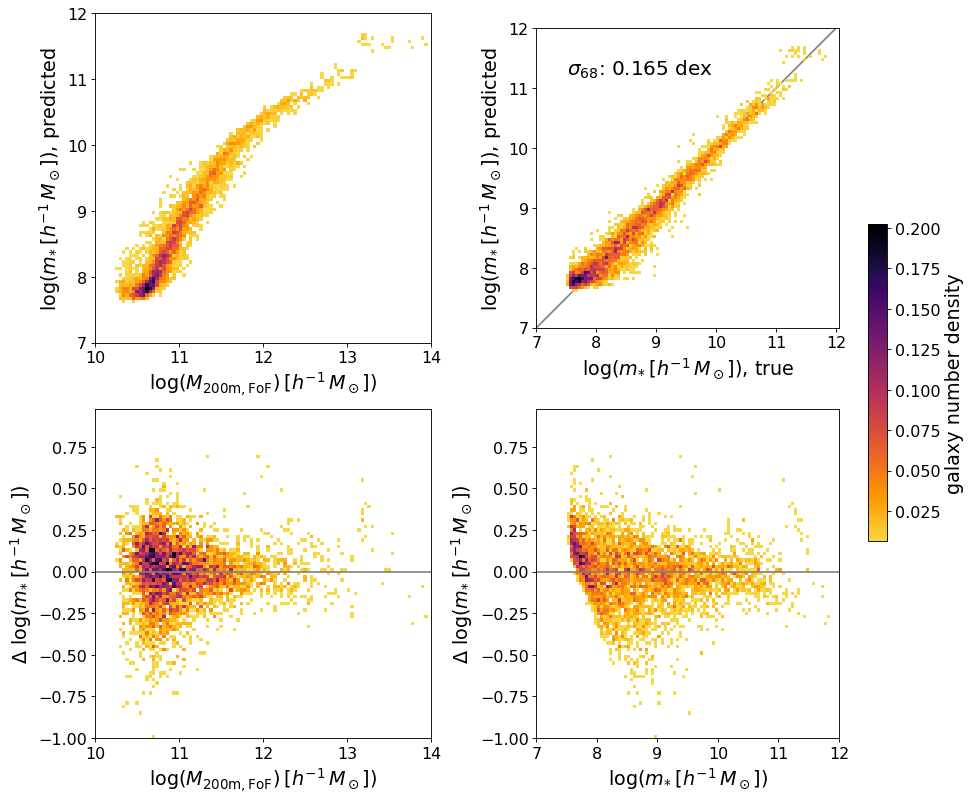
\includegraphics[width=0.7\columnwidth]{pred_mstellar.png}
    \caption{Predictions for the galaxy stellar mass based on the halo shape scalars. The panels show the predicted stellar-to-halo mass relation, the predicted stellar mass compared to the true stellar mass, and the residuals of the stellar mass prediction compared to truth as a function of halo mass.}
    \label{fig:mstellar}
\end{figure}

\begin{figure}
    \centering
    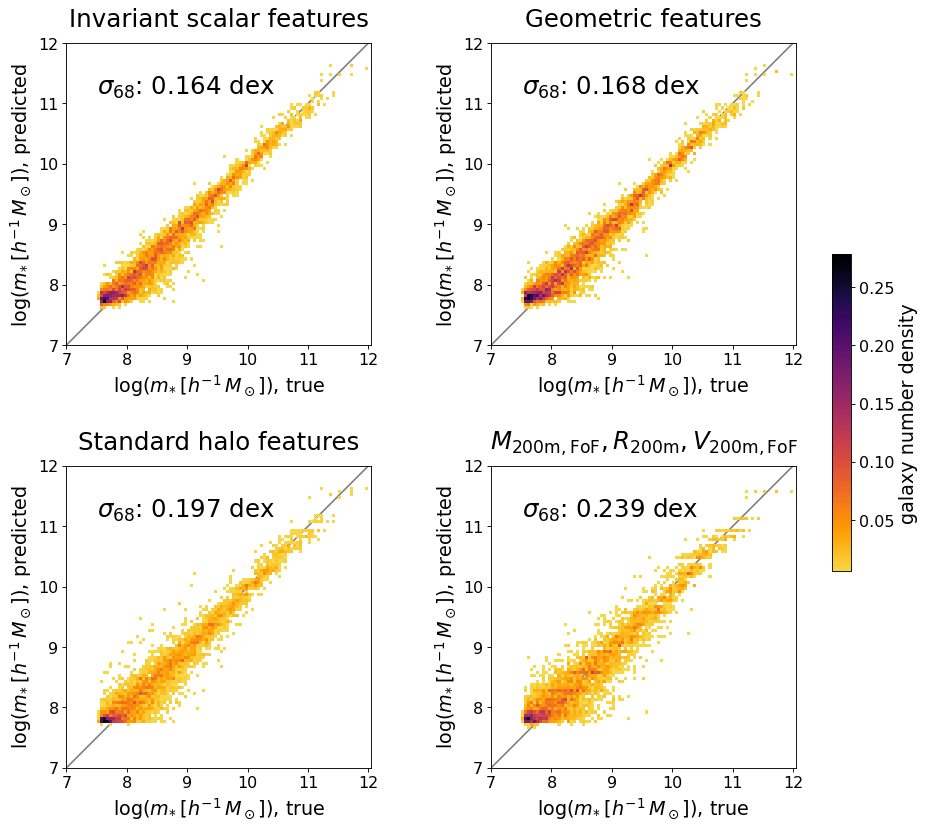
\includegraphics[width=0.7\columnwidth]{feature_comparison_mstellar.png}
    \caption{Predictions for the galaxy stellar mass using the invariant scalars as features, compared to other feature choices: only halo mass, halo summary features, and non-invariant geometric features.}
    \label{fig:mstellar_compare}
\end{figure}


\subsection{Predicting other galaxy properties}

\begin{figure}
    \centering
    \includegraphics[width=0.7\columnwidth]{pred_multi.png}
    \caption{The predicted value of the given galaxy property with our approach, compared to the true value in the matched hydrodynamic simulation. The properties shown are star formation rate, half-mass radius, XXX... . We compare the predictions to those using only the halo summary properties, and using non-invariant geometric features.}
    \label{fig:gal_props}
\end{figure}


\subsection{The mass assembly history encoded in the present-day halo shape}


\begin{figure}
    \centering
    \includegraphics[width=0.5\columnwidth]{pred_mah.png}
    \caption{The predicted mass assembly history of a halo based on the invariant shape scalars. The top panel shows the MAHs of a random selection of halos from the test set, and the predicted scale factor at each mass fraction. The middle panel shows the fractional residuals between the two, and the bottom shows the inner 68th percentile of the predictions for all of our test set, compared to that of the distribution of MAHs used in training. \ksf{rn im plotting test set for latter, make sure to switch to test!}}
    \label{fig:mah}
\end{figure}


\subsection{Understanding the relative importance of the halo shape features}

The feature subsets we consider are: only mass features; mass and position features; mass and velocity features; mass, position and velocity features.
We also investigate limiting to certain orders in $O(x)+O(v)$: 0, 2, and 4.
Finally, we consider different numbers of bins, as well as excluding cross-bins.

\begin{figure}
    \centering
    %\includegraphics{}
    \caption{The precision on the predictions of the given property when using the denoted subset of invariant scalars.}
    \label{fig:features}
\end{figure}


\section{Discussion}
\label{sec:discussion}

Topics/points for discussion section:
\begin{itemize}
    \item Understanding of important features (what do they mean, relationship to currently used features)
    \item Application of approach to useful tasks (constructing mock catalogs, predicting galaxy properties in larger \& higher res simulations and being able to construct many realizations)
    \item The inference problem: going from galaxies to DM
    \item Feature construction choices (e.g. could construct geometric features other ways like with spherical harmonics)
    \item Future goal to move away from halo framework and work on full particle distribution, starting from e.g. density peaks. Intermediate task is to start from halo centers but include all particles, not just those in FoF group
    \item Future work to look at impact of larger-scale environment, incorporate it in input features
    \item Other properties we should predict (position: discuss offsets bw dark and hydro; spin: pseudo-vector)
    \item particles have large time derivative; galaxy has relatively small time derivative! we could show this with our scalars. discuss time dependence.
\end{itemize}


\section{Chapter Acknowledgements}
The authors would like to acknowledge very helpful discussions with Soichiro Hattori, Austen Gabrielpillai, Ben Blum-Smith, Weichi Yao, Scott Tremaine, Rachel Somerville, Derek Lim, and Benjamin Wandelt.
The authors also thank useful feedback by participants of the Flatiron CCA Astrodata Group, Galaxy Formation Group, and Cosmology X Data Science Group.
This research was performed in part at the Coworking Retreat on Equivariant Machine Learning held at the Johns Hopkins University in March 2023.
K.S.F.~is supported by the NASA FINESST program under award number 80NSSC20K1545.
This research made use of computational resources at New York University; we thank the NYU high-performance computing team.